
\begin{figure}[h]
\centering
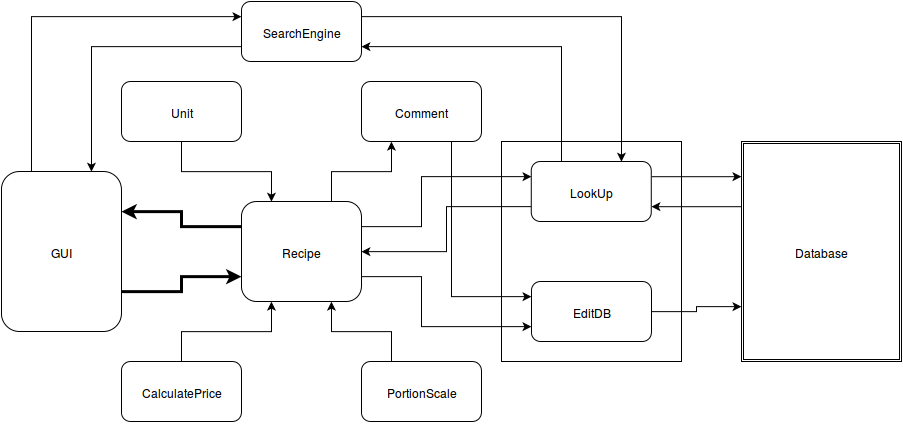
\includegraphics[scale=0.5]{overview.png}
\caption{Översikt över första lagrets moduler.}
\label{fig:overview}
\end{figure}

MatLabb har tre centrala moduler: 
\begin{enumerate}
\item En databas som lagrar all receptrelaterad information.
\item En receptmodul (\verb=Recipe=) som genom hjälpmoduler hämtar, skriver och behandlar databasens information.
\item Ett användargränssnitt (\verb=GUI=) som hjälper användaren att på ett intuitivt och välbekant sätt interagerar med receptmodulen, och i förlängningen databasen.

I detta kapitel ges en överblick över funktionaliteten hos modulerna i första ``lagret'' och hur dessa interagerar.
\end{enumerate}

\section{Databas}\label{sec:ark.databas)}
Databasen utgörs av en MySQL-databas där recept, ingredienser och relaterad data lagras. Exakt data som lagras framgår i kravspecifikationen, samt i kapitel \ref{cha:tekspec} - \emph{Detaljerad teknisk specifikation}.

\section{Recipe}\label{sec:ark.recipe}

\section{GUI}\label{sec:ark.gui}

\section{SearchEngine}\label{sec:ark.search}

\section{Unit}\label{sec:ark.unit}
\verb=Unit= är en modul vars syfte är att konvertera enheter. Den ska kunna hantera prefixbaserade enheter (ex. deciliter $\leftrightarrow$ liter) och bör kunna hantera ``köksmått'' (ex. matsked $\leftrightarrow$ tesked). Modulen ska inte kunna hantera omvandling mellan volymenheter och viktenheter då detta förutsätter känd densitet för ingredienserna i fråga, något som sällan är tillgängligt och av föga intresse.

\verb=Unit= används utav \verb=Recipe= i samspel med \verb=PortionScale=, samt i samspel med \verb=CalculatePrice=.

\section{Comment}\label{sec:ark.comment}
\verb=Comment= är en modul vars syfte är att hantera receptkommentarer. Modulen används utav \verb=Recipe= för att vidarebefodra relevant information till \verb=EditDB=.

\section{CalculatePrice}\label{sec:ark.calcprice}
\verb=CalculatePrice= är en modul som med hjälp av prisdata 

\section{PortionScale}\label{sec:ark.portscale}

\section{Ingredient}\label{sec:ark.ingredient}

\section{LookUp, LookUpIngr}\label{sec:ark.lookup}

\section{EditDB}\label{sec:ark.editdb}

